\documentclass[SCI,english,beameralt]{tumbeamer}

% If you load additional packages, do so in packages.sty as figures are build
% as standalone documents and you may want to have effect on them, too.

% Folder structure:
% .
% ├── beamermods.sty                  % depricated an will be removed soon
% ├── compile                         % remotely compile slides
% ├── figures                         % all figures go here
% │   ├── template              	  % add your figures here
% │   └── final template			  % bottom template
% ├── include                         % create your document here
% │   ├── slides.tex                  % make document wide changes here
% │   ├── intro.tex            		  % introduciton
% │   ├── frameworks.tex              % frameworks
% │   ├── event_model.tex             % event model
% │   ├── summary.tex                 % summary, pros, cons
% │   └── project.tex				  % conclusion and outlook
% ├── lit.bib                         % literature
% ├── Makefile
% ├── packages.sty                    % load additional packages there
% ├── pics                            % binary pcitures go here
% ├── slides.tex                      % main document (may be more than one)
% ├── tumbeamer.cls
% ├── tumcolor.sty                    % TUM color definitions
% ├── tumcontact.sty                  % TUM headers and footers
% ├── tumlang.sty                     % TUM names and language settings
% └── tumlogo.sty                     % TUM logos

% Configure author, title, etc. here:
\usepackage[utf8]{inputenc}
\usepackage{packages}
\usepackage{beamermods}

\usepackage{tikz}
\usepackage{pgfplots}
\usepackage{url}
\usepackage{algorithm2e}
\usepackage{svg}
\usepackage{amsmath}


\author[L. Dickmanns, M. Sellami]{Ludwig Dickmanns, Mahdi Sellami}
\title[Learning Dynamical Systems with NNs]{Learning Dynamical Systems from data: Neural Networks.}

\advisor{Felix Dietrich}


\newdate{date}{23}{01}{2020}
\date{\displaydate{date}}


\usepackage{pgfpages}
\usepackage{ifthen}
% ============================================================================
% jobname solution
% ============================================================================
\newif\ifsolution%
\ifthenelse{\equal{\detokenize{notes}}{\jobname}}{%
\setbeameroption{show notes on second screen=bottom}
\setbeamercolor{note page}{bg=white, fg=black}
\setbeamercolor{note title}{bg=white!95!black, fg=black}
}{
}

% TeXLive 2018 compatibility: https://tex.stackexchange.com/questions/426088/texlive-pretest-2018-beamer-and-subfig-collide
\makeatletter
\let\@@magyar@captionfix\relax
\makeatother


\begin{document}

% If you are preparing a talk but do not like the default font sizes, you may
% want to try the class option 'beameralt', which uses smaller default font
% sizes and integrates subsection/subsubsection names into the headline.

% For lecture mode, you may want to build one set of slides per chapter but
% with common page numbering. If so,
% 1) create a new .tex file for each chapter, e.g. slides_chapN.tex,
% 2) set the part counter to N-1 (assuming chapters start at 0), and
% 3) and name your chapter by using the \part{} command.
%\setcounter{part}{-1}
%\part{Organisatorisches und Einleitung}

% For 16:9 slides, use the class option 'aspectratio=169'.

% If class option 'noframenumbers' is given, frame numbers are not printed.

% If class option 'notitleframe' is given, the title frame is not autmatically
% generated.

% Class option 'nocontentframes' suppresses automatic generation of content
% frames when new parts/sections are started.

% Include source files from ./include (or ./include/chapN).
\section{Introduction}

\begin{frame}
	\frametitle{Overview}
	\begin{itemize}
		\item TASK 1, Summary of the paper contents
		\item TASK 2, Setting up the neural network for Euler's method
		\item TASK 3, Setting up the neural network for the Runge-Kutta method
		\item TASK 4, Testing the networks in dynamical system examples
		\item TASK 5, Construction bifurcation diagrams using the extracted dynamics
	\end{itemize}
\end{frame}

\section{TASK 1, Summary of the paper contents}

\begin{frame}
	\frametitle{Summary}
	\begin{itemize}
		\item Approximation of nonlinear dynamical systems with NNs
		\item Continuous-time models (i.e. sets of ODEs)
		\item Black-Box-Approach
		\begin{itemize}
			\item[$\Rightarrow$] No information on the approximated system
			\item[$\Rightarrow$] The \textbf{entire} system is approximated
		\end{itemize}
		\item Gray-Box-Approach
		\begin{itemize}
			\item[$\Rightarrow$] Some information on the approximated system
			\item[$\Rightarrow$] Only \textbf{unknown} parts of the system are approximated
		\end{itemize}
	\end{itemize}
\end{frame}

\begin{frame}
	\frametitle{Questions}
	\begin{enumerate}
		\item Which integration rule did they use in the paper?
		\begin{itemize}
			\item[$\Rightarrow$] Trapezodial Rule.\vspace{1mm}
			\item[$\Rightarrow$] ODE: $\dot{\overrightarrow{X}} = F(\overrightarrow{X}; \overrightarrow{p})$\vspace{1mm}
			\item[$\Rightarrow$] Rule: $\overrightarrow{X}_{n+1} = \overrightarrow{X}_n + \frac{h}{2}[F(\overrightarrow{X}_n; \overrightarrow{p}) + F(\overrightarrow{X}_{n+1}; \overrightarrow{p})]$
		\end{itemize}
		\item How did they design the neural network?
		\begin{itemize}
			\item[$\Rightarrow$] RNN due to implicit integration rule
			\item[$\Rightarrow$] Two hidden layers with six neurons
			\item[$\Rightarrow$] Sigmodal activation functions
		\end{itemize}
		\item What is the dynamic system used as an illustrative example?
		\begin{itemize}
			\item[$\Rightarrow$] Reactor with a irreversible reaction on a catalytic surface
		\end{itemize}
		\item What are the results?
		\begin{itemize}
			\item[$\Rightarrow$] Good approximations with Gray-Box-Approach
		\end{itemize}
	\end{enumerate}
\end{frame}

\section{Approximated dynamical systems}

\begin{frame}
	\paragraph{Linear system:}\vspace{-2mm}
	\begin{itemize}
		\item[$\Rightarrow$] Two dimensional with no parameter
	\end{itemize}\vspace{-3mm}
	\quad\quad $\dot{x_1} = -0.1 \cdot (x_1 + x_2)$\\
	\quad\quad $\dot{x_2} = 0.25 \cdot x_1$\\
	\vspace{4mm}
	
	\paragraph{Andronov-Hopf system:}\vspace{-2mm}
	\begin{itemize}
		\item[$\Rightarrow$] Two dimensional with one parameter
	\end{itemize}\vspace{-3mm}
	\quad\quad $\dot{x_1} = a \cdot x_1 - x_2 - x_1 \cdot (x_1^2 + x_2^2)$\\
	\quad\quad $\dot{x_2} = x_1 + a \cdot x_2 - x_2 \cdot (x_1^2 + x_2^2)$\\
	\vspace{4mm}
	
	\paragraph{R\"ossler attractor:}\vspace{-2mm}
	\begin{itemize}
		\item[$\Rightarrow$] Three dimensional with one parameter
	\end{itemize}\vspace{-3mm}
	\quad\quad $\dot{x_1} = -x_2 - x_3$\\
	\quad\quad $\dot{x_2} = x_1 + a \cdot x_2$\\
	\quad\quad $\dot{x_3} = 0.2 + x_3 * (x - 14)$
	\vspace{4mm}
\end{frame}
\section{TASK 2, Setting up the neural network for Euler's method}

\begin{frame}
	\frametitle{Euler's Method}
	\paragraph{Formula:}\vspace{-1mm}
	\quad\quad $y_{n+1} = y_n + h \cdot \dot{y}_n$
	\vspace{1mm}
	
	\paragraph{Properties:}\vspace{-2mm}
	\begin{itemize}
		\item Black-Box-Approach
		\item Explicit numerical integration
		\begin{itemize}
			\item[$\Rightarrow$] No RNN required
		\end{itemize}
	\end{itemize}
	
	\paragraph{Architecture}\vspace{2mm}
	\begin{figure}[H]
		\centering
		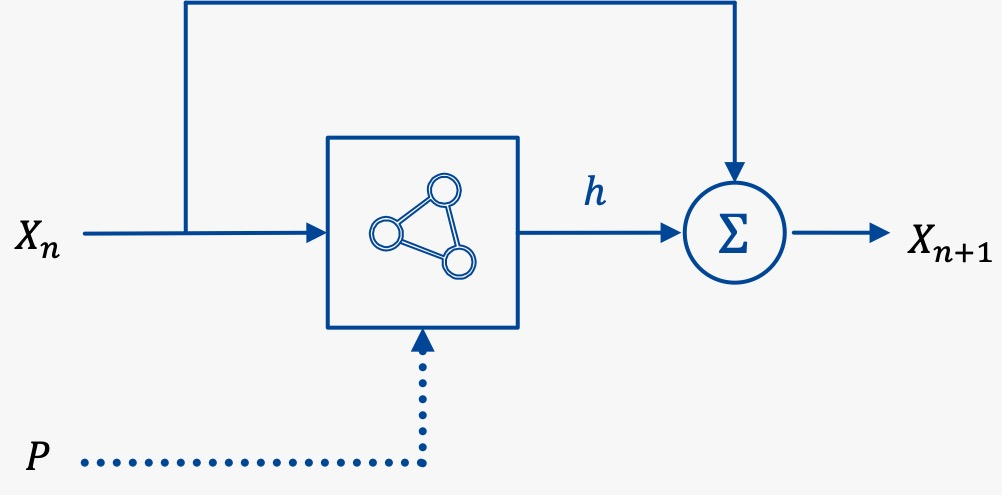
\includegraphics[width=.5\linewidth]{figures/euler/net_architecture}
	\end{figure}
\end{frame}

\begin{frame}
	\frametitle{Network configuration}
	\centering
	\begin{tabular} { c | c | c | c}
						& Linear System & Andronov-Hopf & R\"ossler attractor	\\
		\hline
		Input			& 2 		& 2			& 3			\\
		\hline
		Parameters		& 0 		& 1			& 1			\\
		\hline
		Hidden layers	& 2			& 3			& 3			\\
		\hline
		Neurons / layer	& 20		& 100		& 200		\\
		\hline
		Output			& 2			& 2			& 2			\\
		\hline
		Loss function	& MSE		& MSE		& MSE		\\
		\hline
		Optimization	& SGD		& Adam		& Adam		\\
	\end{tabular}
\end{frame}

\section{TASK 3, Setting up the neural network for the Runge-Kutta method}

\begin{frame}
	\frametitle{Runge-Kutta Method}
	\paragraph{Formula:}
	\quad\quad $y_{n+1} = y_n + h \cdot \sum_{i=1}^s b_i k_i$
	
	\quad\quad $k_i = f \Bigg( t_n + c_i h, y_n + h \cdot \sum_{j=1}^{i-1} a_{ij} k_j\Bigg)$
	\vspace{5mm}
	
	\paragraph{Properties:}\vspace{-2mm}
	\begin{itemize}
		\item Black-Box-Approach
		\item Explicit numerical integration
		\begin{itemize}
			\item[$\Rightarrow$] No RNN required
		\end{itemize}
	\end{itemize}
\end{frame}

\begin{frame}
	\frametitle{Network configuration}
	\centering
	\begin{tabular} { c | c | c | c}
		& Linear System & Andronov-Hopf & R\"ossler attractor	\\
		\hline
		Input			& 2 		& 2			& 3			\\
		\hline
		Parameters		& 0			& 1			& 1			\\
		\hline
		Hidden layers	& 2			& 3			& 3			\\
		\hline
		Neurons / layer	& 20		& 64		& 200		\\
		\hline
		Output			& 2			& 2			& 2			\\
		\hline
		Loss function	& MSE		& MSE		& MSE		\\
		\hline
		Optimization	& SGD		& Adam		& Adam		\\
	\end{tabular}
\end{frame}

\section{TASK 4, Testing the networks}

\begin{frame}
	\frametitle{Euler's method -- linear system}
	\paragraph{Dataset}\vspace{-2mm}
	\begin{itemize}
		\item 1 Mio. random samples of $\overrightarrow{x}_{n}$ and $\overrightarrow{x}_{n+1}$
		\item Samples between $-100$ and $100$ (both $x_1$ and $x_2$)
	\end{itemize}
	\paragraph{Trajectories}\vspace{-2mm}
	\begin{figure}[H]
		\subfloat[$x_0 = (100, -100)$]{
			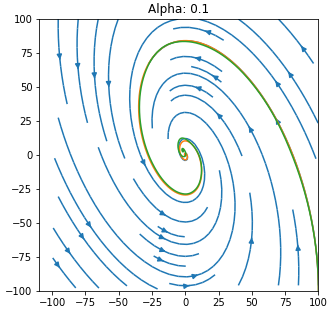
\includegraphics[width=.30\linewidth]{figures/euler/ls_100_-100.png}
		}\quad
		\subfloat[$x_0 = (-75, 100)$]{
			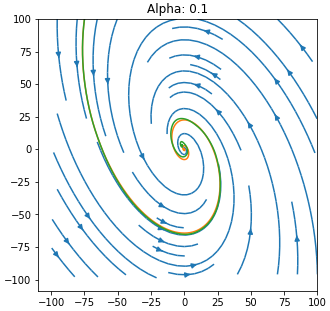
\includegraphics[width=.30\linewidth]{figures/euler/ls_-75_100.png}
		}\quad
		\subfloat[$x_0 = (-100, 25)$]{
			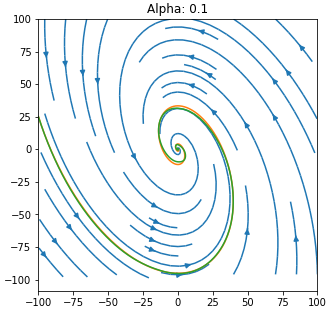
\includegraphics[width=.30\linewidth]{figures/euler/ls_-100_25.png}
		}
		\caption{Phase diagrams for different values of $x_0$.}
	\end{figure}
\end{frame}

\begin{frame}
	\frametitle{Euler's method -- Andronov-Hopf system}
	\paragraph{Dataset}\vspace{-2mm}
	\begin{itemize}
		\item 1000 trajectories
		\item Trajectories starting between $-5$ and $5$ (both $x_1$ and $x_2$)
		\item $alpha$ values between $-3$ and $3$
	\end{itemize}
	\paragraph{Trajectories}\vspace{-2mm}
	\begin{figure}[H]
		\subfloat[$x_0 = (2, -2)$; $alpha = -1$]{
			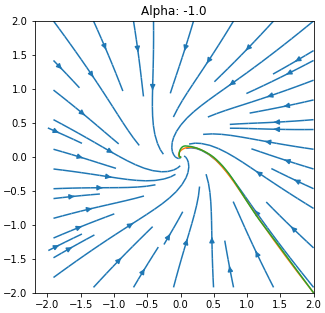
\includegraphics[width=.30\linewidth]{figures/euler/and_hopf_a_-1.png}
		}\quad
		\subfloat[$x_0 = (2, -2)$; $alpha = 0$]{
			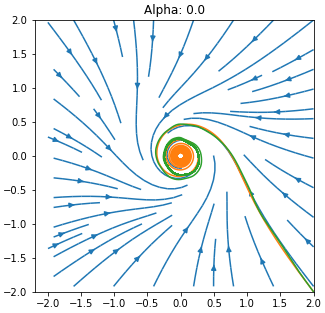
\includegraphics[width=.30\linewidth]{figures/euler/and_hopf_a_0.png}
		}\quad
		\subfloat[$x_0 = (2, -1)$; $alpha = 1$]{
			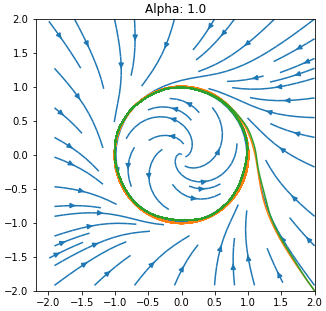
\includegraphics[width=.30\linewidth]{figures/euler/and_hopf_a_1.png}
		}
		\caption{Phase diagrams for different values of $alpha$.}
	\end{figure}
\end{frame}

\begin{frame}
	\frametitle{Euler's method -- R\"ossler attractor}
	\paragraph{Dataset}\vspace{-2mm}
	\begin{itemize}
		\item 150 trajectories
		\item Trajectories starting between $0$ and $10$ (for $x_1$, $x_2$ and $x_3$)
		\item $a$ values between $-0.1$ and $0.3$
	\end{itemize}
	\paragraph{Trajectories}\vspace{-2mm}
	\begin{figure}[H]
		\subfloat[$x_0 = (5, 5, 5)$; $a = -0.1$]{
			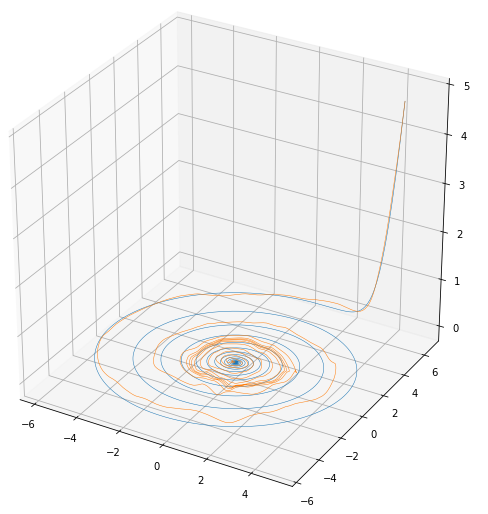
\includegraphics[width=.35\linewidth]{figures/euler/roe_-0_1.png}
		}\quad
		\subfloat[$x_0 = (5, 5, 5)$; $a = 0.0$]{
			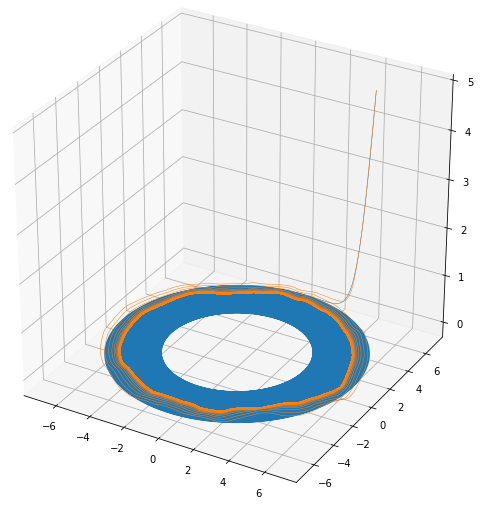
\includegraphics[width=.35\linewidth]{figures/euler/roe_0_0.png}
		}
		\caption{Phase diagrams for different values of $a$.}
	\end{figure}
\end{frame}

\begin{frame}
	\frametitle{Euler's method -- R\"ossler attractor}
	\paragraph{Trajectories}\vspace{-1mm}
	\begin{figure}[H]
		\subfloat[$x_0 = (5, 5, 5)$; $a = 0.1$]{
			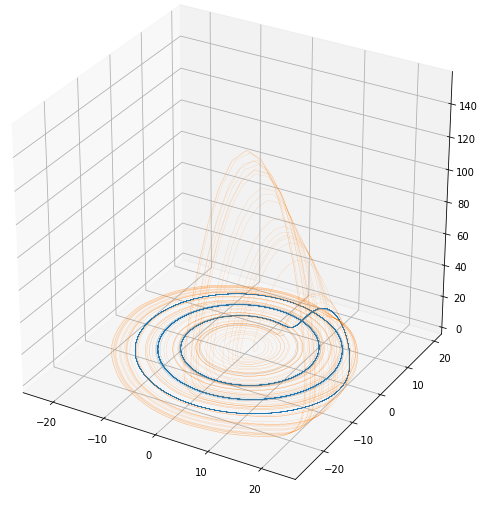
\includegraphics[width=.30\linewidth]{figures/euler/roe_0_1.png}
		}\quad
		\subfloat[$x_0 = (5, 5, 5)$; $a = 0.2$]{
			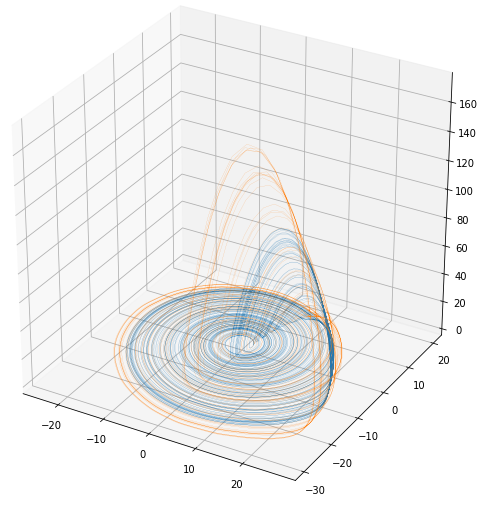
\includegraphics[width=.30\linewidth]{figures/euler/roe_0_2.png}
		}\quad
		\subfloat[$x_0 = (5, 5, 5)$; $a = 0.3$]{
			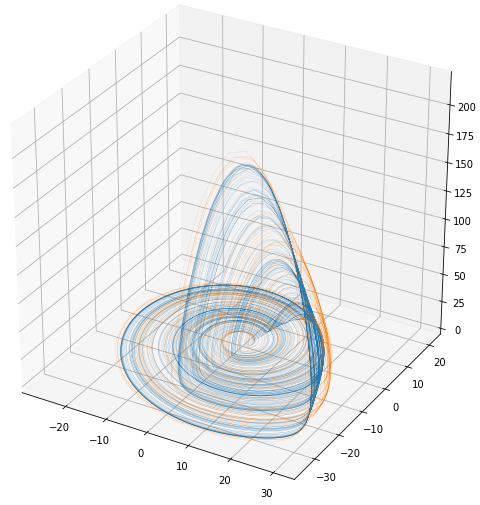
\includegraphics[width=.30\linewidth]{figures/euler/roe_0_3.png}
		}
		\caption{Phase diagrams for different values of $a$.}
	\end{figure}
\end{frame}

\begin{frame}
	\frametitle{Runge-Kutta method -- linear system}
	\paragraph{Dataset}\vspace{-2mm}
	\begin{itemize}
		\item 1 Mio. random samples of $\overrightarrow{x}_{n}$ and $\overrightarrow{x}_{n+1}$
		\item Samples between $-100$ and $100$ (both $x_1$ and $x_2$)
	\end{itemize}
	\paragraph{Trajectories}\vspace{-2mm}
	\begin{figure}[H]
		\subfloat[$x_0 = (100, -100)$]{
			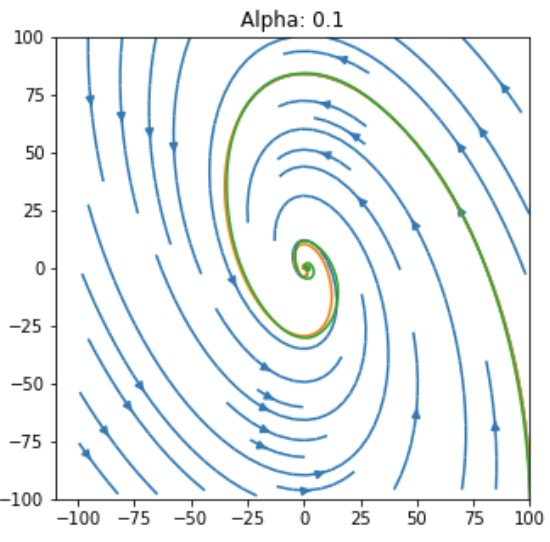
\includegraphics[width=.30\linewidth]{figures/runge_kutta/ls_100_-100.png}
		}\quad
		\subfloat[$x_0 = (-75, 100)$]{
			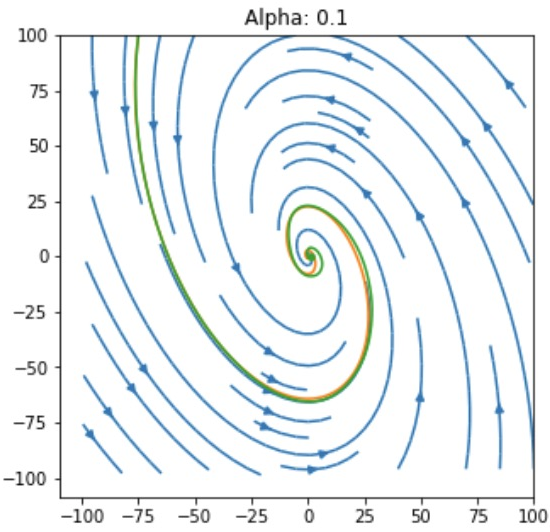
\includegraphics[width=.30\linewidth]{figures/runge_kutta/ls_-75_100.png}
		}\quad
		\subfloat[$x_0 = (-100, 25)$]{
			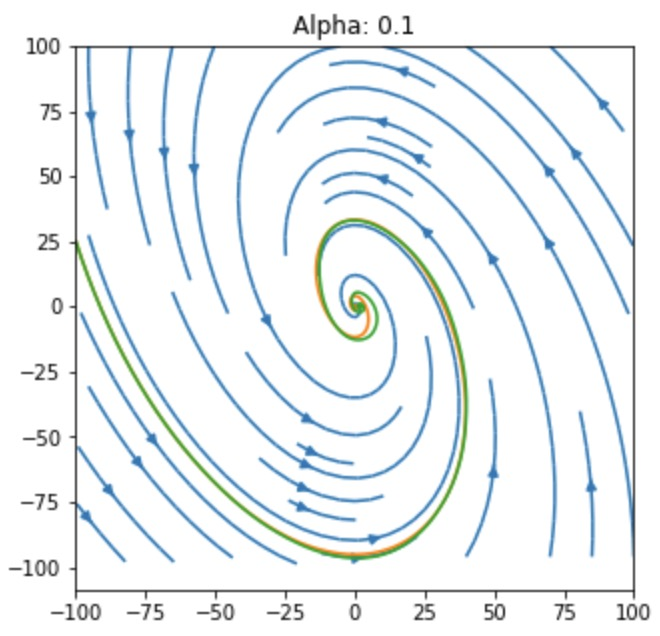
\includegraphics[width=.30\linewidth]{figures/runge_kutta/ls_-100_25.png}
		}
		\caption{Phase diagrams for different values of $x_0$.}
	\end{figure}
\end{frame}

\begin{frame}
	\frametitle{Runge-Kutta method -- Andronov-Hopf system}
	\paragraph{Dataset}\vspace{-2mm}
	\begin{itemize}
		\item 1000 trajectories
		\item Trajectories starting between $-5$ and $5$ (both $x_1$ and $x_2$)
	\end{itemize}
	\paragraph{Trajectories}\vspace{-2mm}
	\begin{figure}[H]
		\subfloat[$x_0 = (2, -2)$; $alpha = -1$]{
			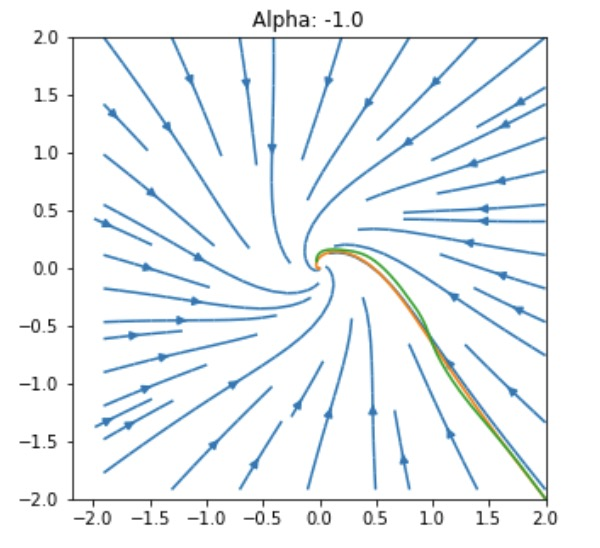
\includegraphics[width=.30\linewidth]{figures/runge_kutta/and_hopf_a_-1.png}
		}\quad
		\subfloat[$x_0 = (2, -2)$; $alpha = 0$]{
			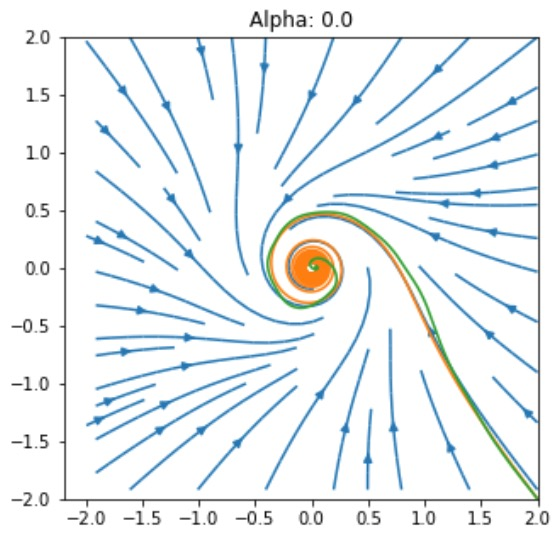
\includegraphics[width=.30\linewidth]{figures/runge_kutta/and_hopf_a_0.png}
		}\quad
		\subfloat[$x_0 = (2, -2)$; $alpha = 1$]{
			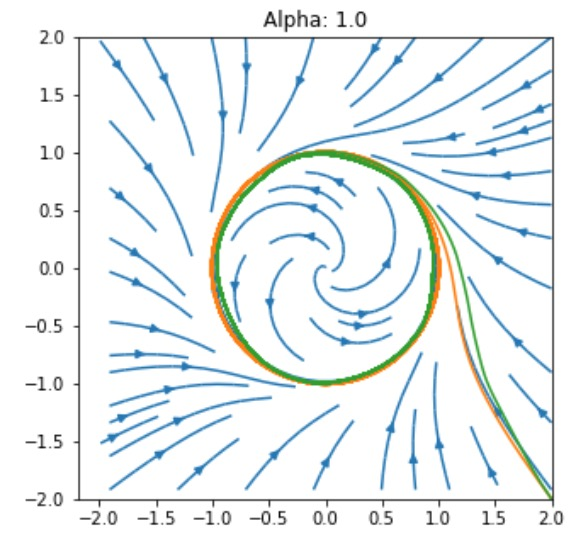
\includegraphics[width=.30\linewidth]{figures/runge_kutta/and_hopf_a_1.png}
		}
		\caption{Phase diagrams for different values of $alpha$.}
	\end{figure}
\end{frame}

\begin{frame}
	\frametitle{Runge-Kutta method -- R\"ossler attractor}
	\paragraph{Dataset}\vspace{-2mm}
	\begin{itemize}
		\item 150 trajectories
		\item Trajectories starting between $0$ and $10$ (for $x_1$, $x_2$ and $x_3$)
		\item $a$ values between $-0.1$ and $0.3$
	\end{itemize}
	\paragraph{Trajectories}\vspace{-2mm}
	\begin{figure}[H]
		\subfloat[$x_0 = (5, 5, 5)$; $a = -0.1$]{
			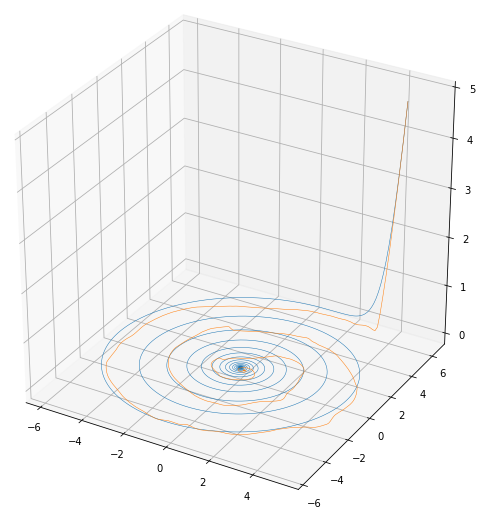
\includegraphics[width=.35\linewidth]{figures/runge_kutta/roe_-0_1.png}
		}\quad
		\subfloat[$x_0 = (5, 5, 5)$; $a = 0.0$]{
			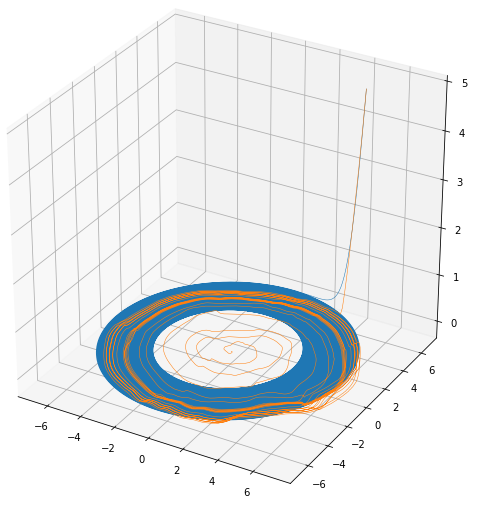
\includegraphics[width=.35\linewidth]{figures/runge_kutta/roe_0_0.png}
		}
		\caption{Phase diagrams for different values of $a$.}
	\end{figure}
\end{frame}

\begin{frame}
	\frametitle{Runge-Kutta method -- R\"ossler attractor}
	\paragraph{Trajectories}\vspace{-1mm}
	\begin{figure}[H]
		\subfloat[$x_0 = (5, 5, 5)$; $a = 0.1$]{
			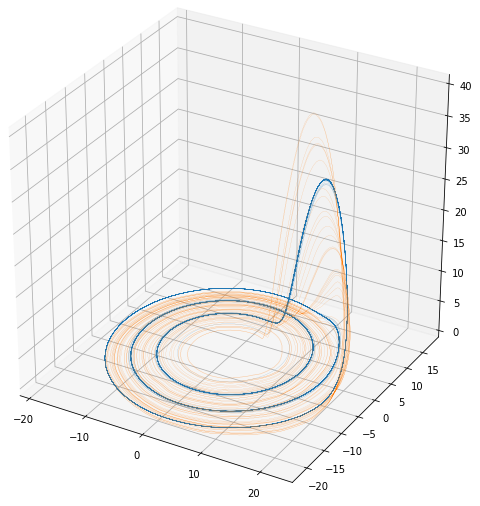
\includegraphics[width=.30\linewidth]{figures/runge_kutta/roe_0_1.png}
		}\quad
		\subfloat[$x_0 = (5, 5, 5)$; $a = 0.2$]{
			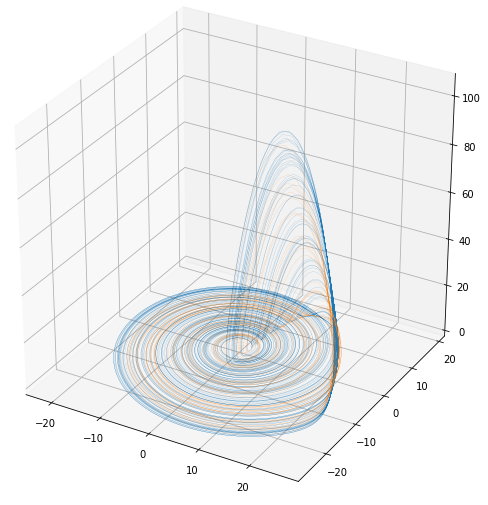
\includegraphics[width=.30\linewidth]{figures/runge_kutta/roe_0_2.png}
		}\quad
		\subfloat[$x_0 = (5, 5, 5)$; $a = 0.3$]{
			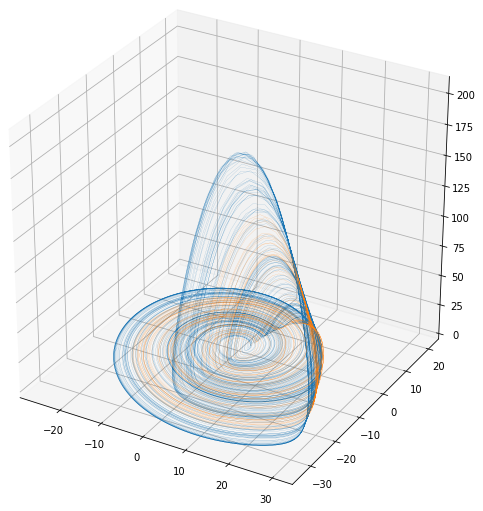
\includegraphics[width=.30\linewidth]{figures/runge_kutta/roe_0_3.png}
		}
		\caption{Phase diagrams for different values of $a$.}
	\end{figure}
\end{frame}

\section{TASK 5, Constructing bifurcation diagrams}

\begin{frame}
	\frametitle{Euler's method -- Andronov-Hopf system}
	\paragraph{Data}\vspace{-4mm}
	\begin{figure}[H]
		\subfloat{
			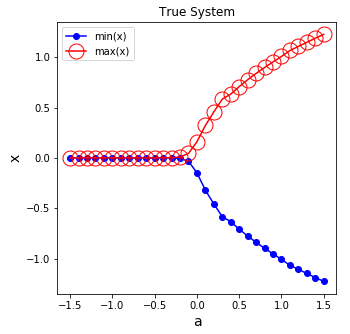
\includegraphics[width=.28\linewidth]{figures/euler/bifurcation/true_and_hopf_x.png}
		}\quad
		\subfloat{
			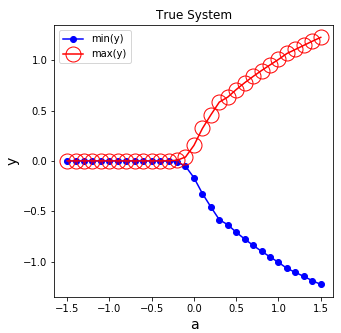
\includegraphics[width=.28\linewidth]{figures/euler/bifurcation/true_and_hopf_y.png}
		}
	\end{figure}
	\paragraph{Approximation}\vspace{-4mm}
	\begin{figure}[H]
		\subfloat{
			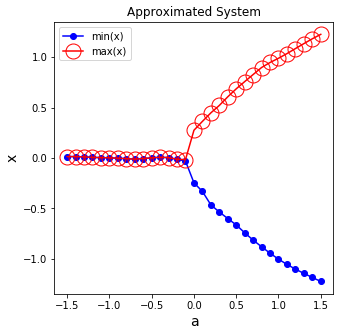
\includegraphics[width=.28\linewidth]{figures/euler/bifurcation/approx_and_hopf_x.png}
		}\quad
		\subfloat{
			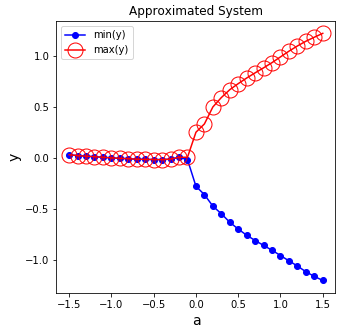
\includegraphics[width=.28\linewidth]{figures/euler/bifurcation/approx_and_hopf_y.png}
		}
	\end{figure}
\end{frame}

\begin{frame}
	\frametitle{Euler's method -- R\"ossler attractor}
	\paragraph{Data}\vspace{-4mm}
	\begin{figure}[H]
		\subfloat{
			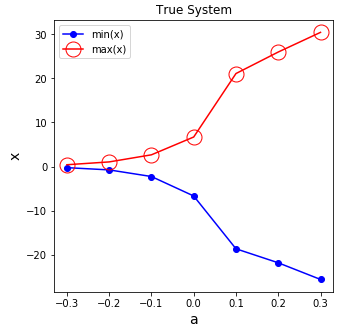
\includegraphics[width=.28\linewidth]{figures/euler/bifurcation/true_roe_x.png}
		}\quad
		\subfloat{
			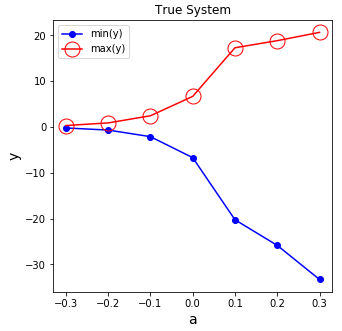
\includegraphics[width=.28\linewidth]{figures/euler/bifurcation/true_roe_y.png}
		}\quad
		\subfloat{
			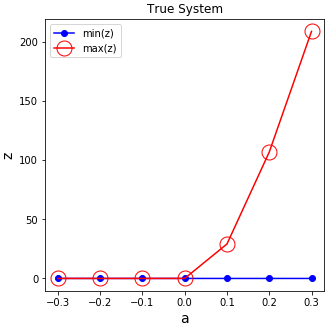
\includegraphics[width=.28\linewidth]{figures/euler/bifurcation/true_roe_z.png}
		}
	\end{figure}
	\paragraph{Approximation}\vspace{-4mm}
	\begin{figure}[H]
		\subfloat{
			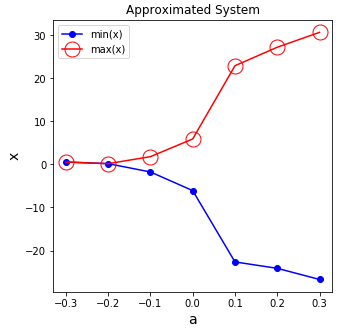
\includegraphics[width=.28\linewidth]{figures/euler/bifurcation/approx_roe_x.png}
		}\quad
		\subfloat{
			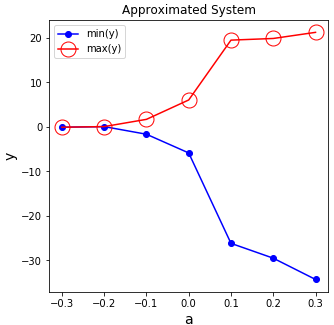
\includegraphics[width=.28\linewidth]{figures/euler/bifurcation/approx_roe_y.png}
		}\quad
		\subfloat{
			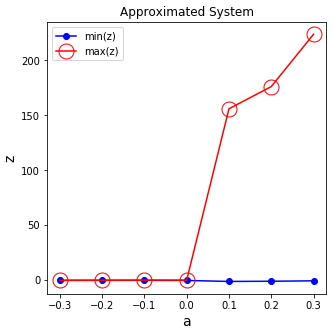
\includegraphics[width=.28\linewidth]{figures/euler/bifurcation/approx_roe_z.png}
		}
	\end{figure}
\end{frame}

\begin{frame}
\frametitle{Runge-Kutta method -- Andronov-Hopf system}
	\paragraph{Data}\vspace{-4mm}
	\begin{figure}[H]
		\subfloat{
			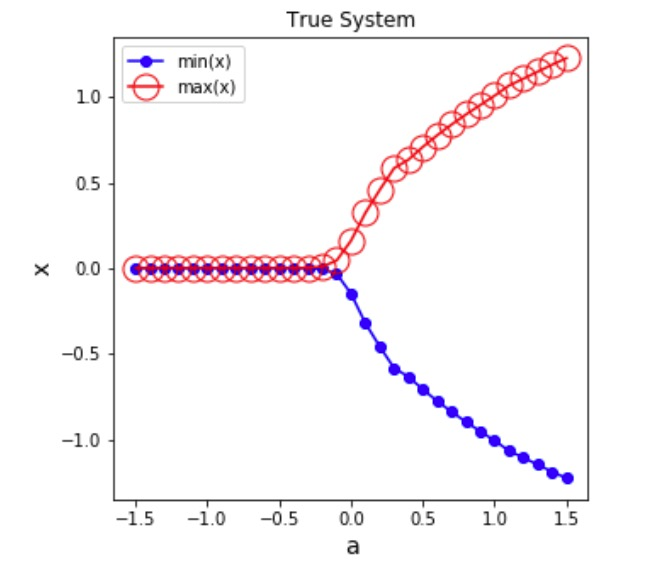
\includegraphics[width=.28\linewidth]{figures/runge_kutta/bifurcation/true_and_hopf_x.png}
		}\quad
		\subfloat{
			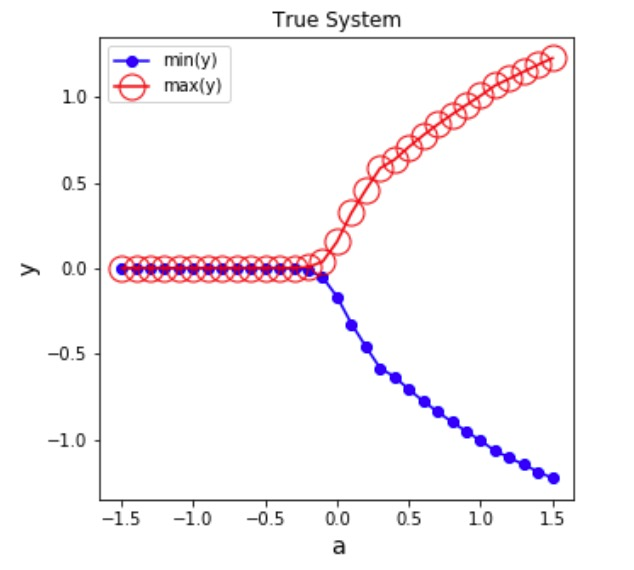
\includegraphics[width=.28\linewidth]{figures/runge_kutta/bifurcation/true_and_hopf_y.png}
		}
	\end{figure}
	\paragraph{Approximation}\vspace{-4mm}
	\begin{figure}[H]
		\subfloat{
			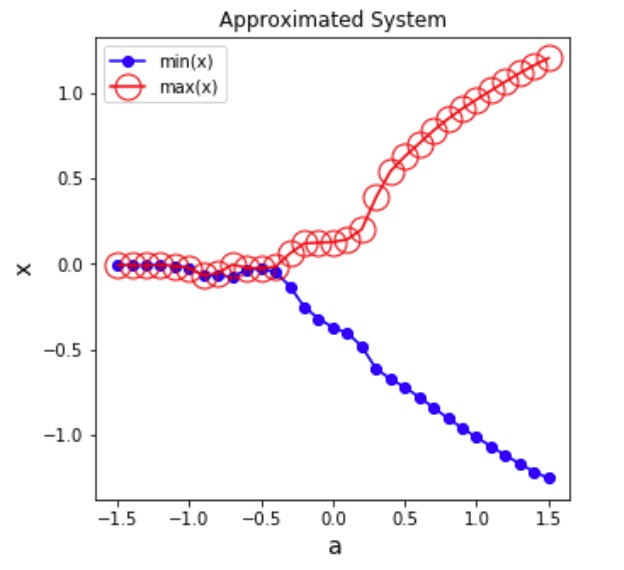
\includegraphics[width=.28\linewidth]{figures/runge_kutta/bifurcation/approx_and_hopf_x.png}
		}\quad
		\subfloat{
			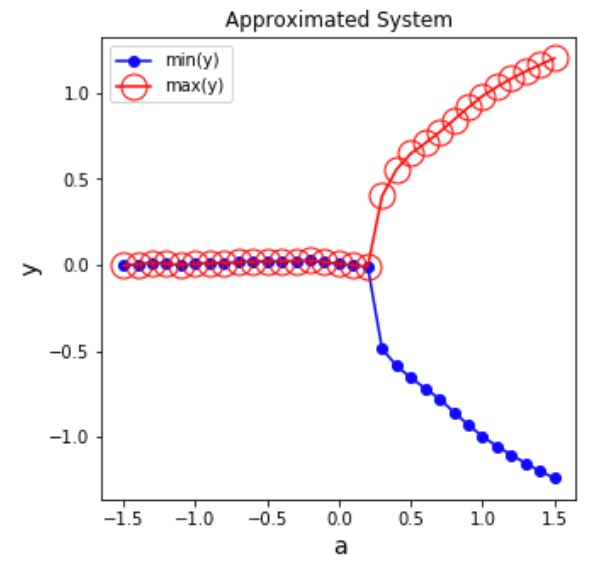
\includegraphics[width=.28\linewidth]{figures/runge_kutta/bifurcation/approx_and_hopf_y.png}
		}
	\end{figure}
\end{frame}

\begin{frame}
	\frametitle{Runge-Kutta method -- R\"ossler attractor}
	\paragraph{Data}\vspace{-4mm}
	\begin{figure}[H]
		\subfloat{
			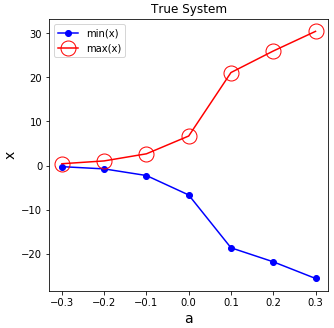
\includegraphics[width=.28\linewidth]{figures/runge_kutta/bifurcation/true_roe_x.png}
		}\quad
		\subfloat{
			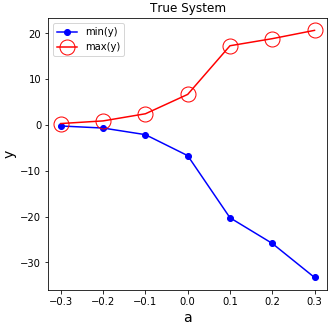
\includegraphics[width=.28\linewidth]{figures/runge_kutta/bifurcation/true_roe_y.png}
		}\quad
		\subfloat{
			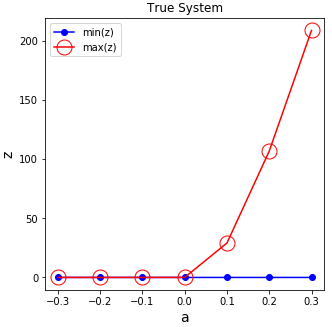
\includegraphics[width=.28\linewidth]{figures/runge_kutta/bifurcation/true_roe_z.png}
		}
	\end{figure}
	\paragraph{Approximation}\vspace{-4mm}
	\begin{figure}[H]
		\subfloat{
			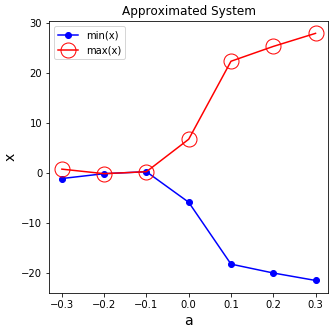
\includegraphics[width=.28\linewidth]{figures/runge_kutta/bifurcation/approx_roe_x.png}
		}\quad
		\subfloat{
			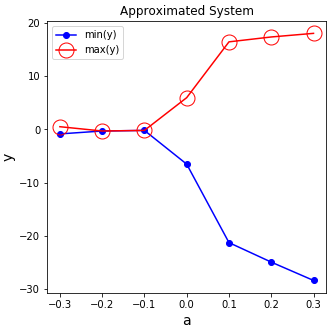
\includegraphics[width=.28\linewidth]{figures/runge_kutta/bifurcation/approx_roe_y.png}
		}\quad
		\subfloat{
			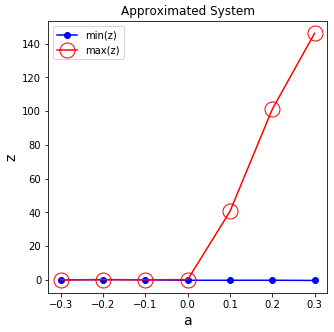
\includegraphics[width=.28\linewidth]{figures/runge_kutta/bifurcation/approx_roe_z.png}
		}
		\end{figure}
\end{frame}


\section{Conclusion}

\begin{frame}
	\frametitle{Summary}
	\begin{itemize}
		\item Very good results for linear and Andronov-Hopf systems
		\item Not as, but still good results for R\"ossler attractor
		\item Not only the dynamics, but also the parameters could be learned quite well
		\item Well approximation of dynamical systems \textbf{just} from data via NNs
	\end{itemize}
\end{frame}

\begin{frame}
	\centering
	\paragraph{Thanks for your attention!}
\end{frame}

\begin{frame}
	\centering
	\paragraph{Questions?}
\end{frame}


% Comment out if you do not want a bibliography
%\section{Bibliography}
%\begin{frame}[allowframebreaks]
%    \bibliographystyle{abbrv}
%    \setbeamertemplate{bibliography item}[text]
%    \footnotesize
%    \bibliography{lit}
%\end{frame}

\end{document}

